\newpage
%\pagestyle{empty}

\begin{minipage}[c]{.25\linewidth}
	
\includegraphics[width=4cm]{images/Logo-LEnsE.png}
\end{minipage} \hfill
\begin{minipage}[c]{.4\linewidth}

\begin{center}
\vspace{0.3cm}
{\Large \textsc{Interféromètre de ZYGO}}

\medskip

\textbf{\Large IHM - \textsc{Acquisition}}

\end{center}
\end{minipage}\hfill

%%%%%%%%%%%%%%%%%%%%%%%%%%%%%%%%%%
%%%%%%%%%%%%%%%%%%%%%%%%%%%%%%%%%%
\section{Acquisition d'une série d'interférogrammes}

La première étape avant de pouvoir analyser l'état de surface des optiques est l'\textbf{acquisition des interférogrammes} à différentes positions.

Cette étape se fait dans la partie \mbox{\fbox{\textbf{\textsc{Acquisition}}}} de l'application.

\medskip

Cette section regroupe les sous-mode suivant :

\begin{description}
	\item[\mbox{\fbox{Caméra}}] qui permet de modifier le temps d'exposition et le niveau de noir de la caméra Basler du système
	\item[\mbox{\fbox{Gestion du piezo}}] qui permet de valider le fonctionnement de la cale piézoélectrique
	\item[\mbox{\fbox{Acquisition Simple}}] qui permet de lancer une nouvelle acquisition d'interférogramme (5 images déphasées de $\lambda/4$.
\end{description}


%%%%%%%%%%%%%%%%%%%%%%%%%%%%%%%%%%
\subsection{Caméra}

La section \mbox{\fbox{\textsc{\textbf{Caméra}}}} permet de lancer la \textbf{visualisation de l'interférogramme} (en mode \textsc{View}).

Un \textbf{histogramme} ainsi qu'une \textbf{coupe au centre de l'image} sont affichés dans la partie de droite. 

\medskip

Il est possible de régler le \textbf{temps d'exposition} et le \textbf{niveau de noir} (offset des pixels) de la caméra. 

\medskip

Le \textbf{niveau de noir} doit être réglé pour que les franges sombres ne soient pas écrêtées vers le bas (autour de 0) sur la coupe tout en maintenant un niveau proche de 0 en terme de luminisité.

Le \textbf{temps d'exposition} doit être réglé pour que les franges claires ne soient pas écrêtées vers le haut (autour de 255) sur la coupe tout en garantissant la meilleure dynamique possible sur la caméra.

\medskip


\begin{center}
	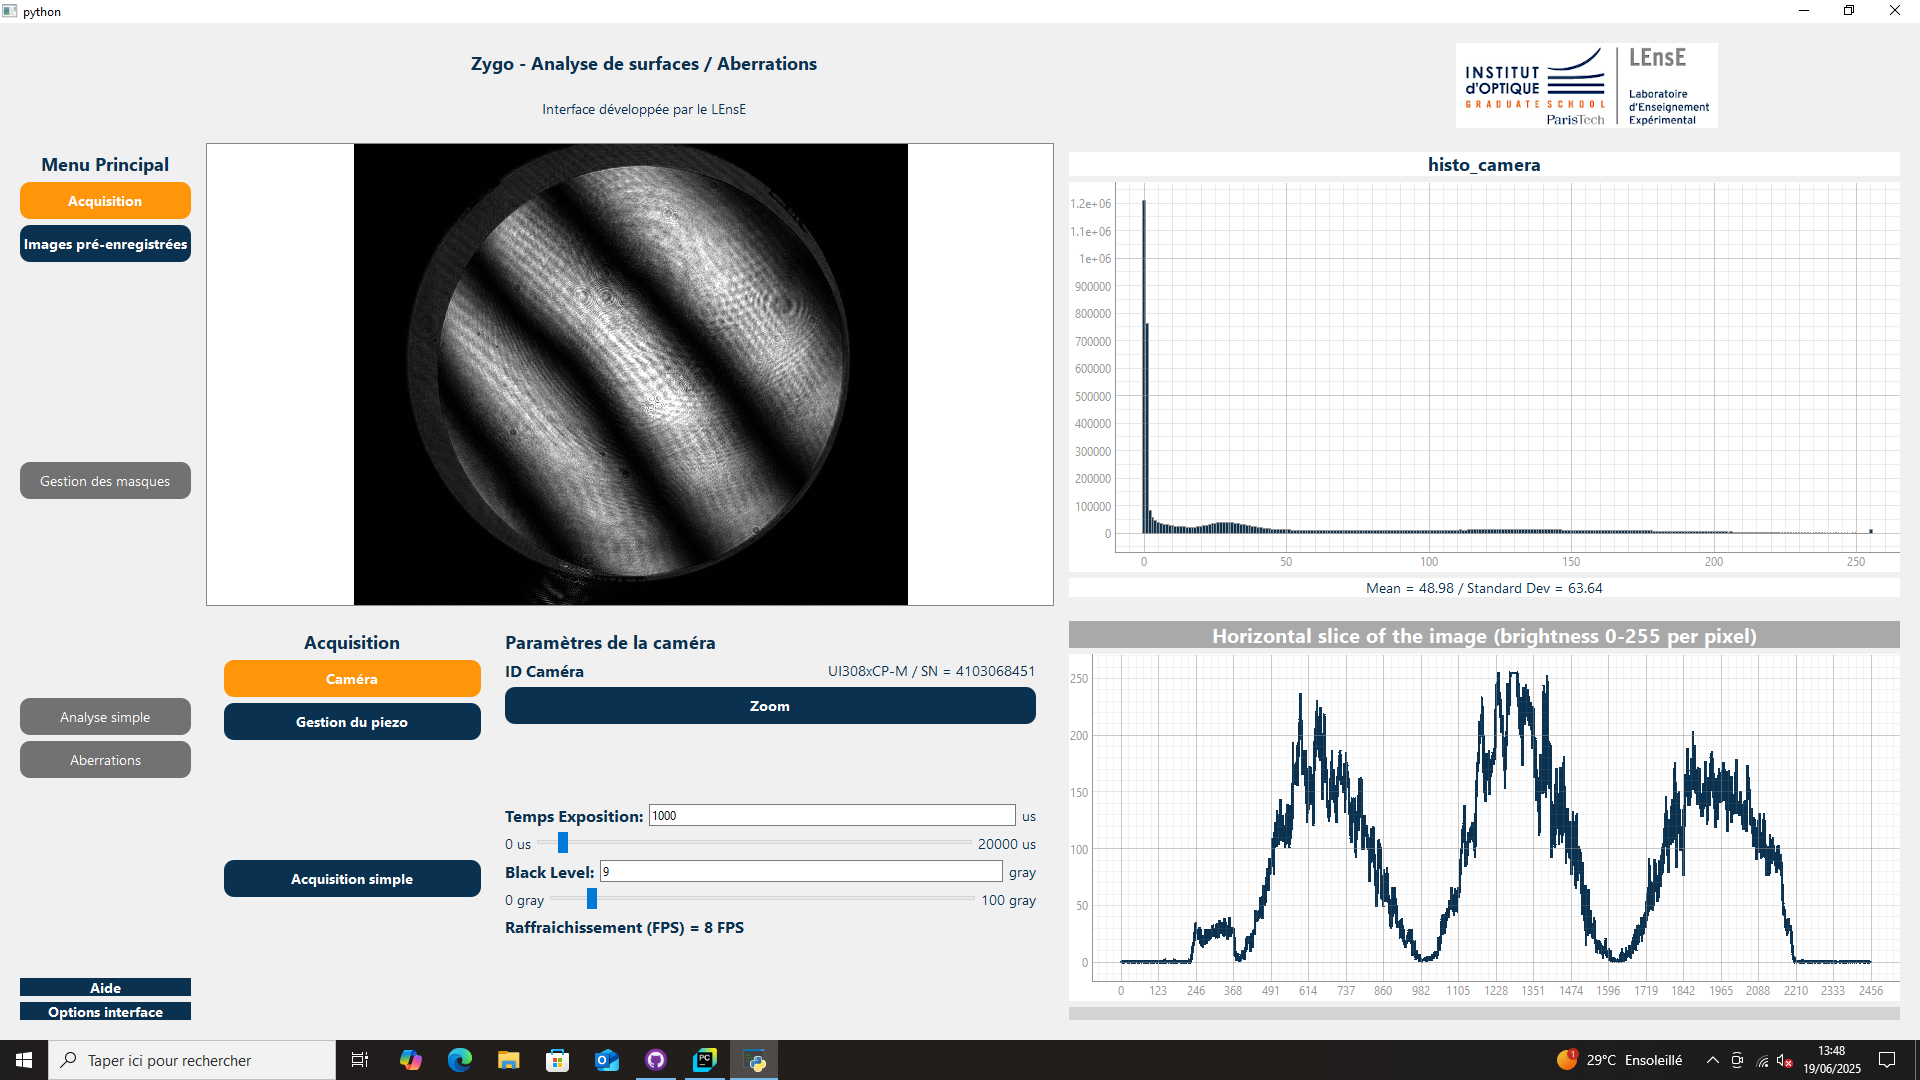
\includegraphics[width=0.9\textwidth]{images/zygo_acquisition_camera.png}
\end{center}

\newpage

%%%%%%%%%%%%%%%%%%%%%%%%%%%%%%%%%%
\subsection{Acquisition Simple}

La section \mbox{\fbox{\textsc{\textbf{Acquisition Simple}}}} permet de lancer l'\textbf{acquisition de 5 interférogrammes}.

\medskip

Il faut cliquer sur l'un des deux boutons \mbox{\fbox{\textsc{Lancer l'acquisition}}}.

Le \textbf{premier bouton} supprime tous les masques en mémoire.

Le \textbf{second bouton} conserve l'ensemble des masques déjà pré-établis.

\medskip

Une barre de progression permet de connaître l'état d'avancement de l'acquisition. Cette phase dure quelques secondes.

\bigskip

Lorsque l'acquisition est terminée, une série de 6 images s'affiche dans la partie de droite : les 5 premières images correspondent à chaque interférogramme déphasé de $\lambda/4$ et la dernière (en bas à droite) correspond à la somme des 4 premières.

La dernière image doit montrer une teinte quasiment plate dans la zone d'étude.


\begin{center}
	
\includegraphics[width=0.9\textwidth]{images/zygo_acquisition_simple.png}
\end{center}

%%%%%%%%%%%%%%%%%%%%%%%%%%%%%%%%%%
\subsection{Gestion de la cale piézoélectrique}

La section \mbox{\fbox{\textsc{\textbf{Gestion du piezo}}}} permet de \textbf{modifier la tension appliquée à la cale piézoélectrique}, permettant de changer le chemin optique et ainsi déplacer les franges de l'interférogramme.

IMAGES pour V=1V, V=2V, V=3V ?
